\documentclass[10pt,a4paper]{article}
\usepackage[utf8]{inputenc}
\usepackage{fullpage}
\usepackage{graphicx}
\usepackage{fancyhdr}
\usepackage{occi}
\setlength{\headheight}{13pt}
\pagestyle{fancy}

\newcommand{\doccode}{XXXXX}

% default sans-serif
\renewcommand{\familydefault}{\sfdefault}

% no lines for headers and footers
\renewcommand{\headrulewidth}{0pt}
\renewcommand{\footrulewidth}{0pt}

% header
\fancyhf{}
\lhead{\doccode}
\rhead{\today}

% footer
\lfoot{occi-wg@ogf.org}
\rfoot{\thepage}

% paragraphs need some space...
\setlength{\parindent}{0pt}
\setlength{\parskip}{1ex plus 0.5ex minus 0.2ex}

% some space between header and text...
\headsep 13pt

\setcounter{secnumdepth}{4}

\begin{document}

% header on first page is different
\thispagestyle{empty}

\doccode \hfill Augusto Ciuffoletti, Univ. of Pisa\\ 
OCCI-WG \hfill Thijs Metsch, Intel Corp.\\
\rightline {Andy Edmonds, Zurich University of Applied Sciences}\\
\rightline {September 22, 2014}\\
\rightline {Updated: \today}

\vspace*{0.5in}

\begin{Large}
\textbf{Open Cloud Computing Interface - Notification Extension}
\end{Large}

\vspace*{0.5in}

\underline{Status of this Document}

This document provides information to the community regarding the
specification of the Open Cloud Computing Interface. Distribution is
unlimited.

\underline{Copyright Notice}

Copyright \copyright ~Open Grid Forum (2009-2011). All Rights Reserved.

\underline{Trademarks}

OCCI is a trademark of the Open Grid Forum.

\underline{Abstract}

This document, part of a document series, produced by the OCCI working
group within the Open Grid Forum (OGF), provides a high-level
definition of a Protocol and API. The document is based upon
previously gathered requirements and focuses on the scope of important
capabilities required to support modern service offerings.


\newpage
\tableofcontents
\newpage

\section{Introduction}
The Open Cloud Computing Interface (OCCI) is a RESTful Protocol and
API for all kinds of management tasks. OCCI was originally initiated
to create a remote management API for IaaS%
\footnote{Infrastructure as a Service}
model-based services, allowing for the development of interoperable tools for
common tasks including deployment, autonomic scaling and monitoring.
%
It has since evolved into a flexible API with a strong focus on
interoperability while still offering a high degree of extensibility. The
current release of the Open Cloud Computing Interface is suitable to serve many
other models in addition to IaaS, including PaaS and SaaS.

In order to be modular and extensible the current OCCI specification is
released as a suite of complimentary documents, which together form the complete
specification.
%
The documents are divided into four categories consisting of the OCCI Core,
the OCCI Protocols, the OCCI Renderings and the OCCI Extensions.
%
\begin{itemize}
\item The OCCI Core specification consists of a single document defining the
 OCCI Core Model. The OCCI Core Model can be interacted with through {\em
 renderings} (including associated behaviors) and expanded through {\em extensions}.
\item The OCCI Protocol specifications consist of multiple documents, each
 describing how the model can be interacted with over a particular protocol (e.g. HTTP, AMQP etc.).
 Multiple protocols can interact with the same instance of the OCCI Core Model.
\item The OCCI Rendering specifications consist of multiple documents, each
 describing a particular rendering of the OCCI Core Model. Multiple renderings can
 interact with the same instance of the OCCI Core Model and will automatically support
 any additions to the model which follow the extension rules defined in OCCI
 Core.
\item The OCCI Extension specifications consist of multiple documents,
  each describing a particular extension of the OCCI Core Model. The
  extension documents describe additions to the OCCI Core Model
  defined within the OCCI specification suite.
\end{itemize}
%

The current specification consists of seven documents. This
specification describes version 1.2 of OCCI and is backward compatible with 1.1.
Future releases of OCCI
may include additional protocol, rendering and extension specifications. The specifications to be
implemented (MUST, SHOULD, MAY) are detailed in the table below.

\mytablefloat{
	\label{tbl:occi_compliancy}%
	What OCCI specifications must be implemented for the specific version.
}
{
	\begin{tabular}{lll}
	\toprule
	Document & OCCI 1.1 & OCCI 1.2 \\
	\colrule
	Core Model & MUST & MUST \\
	Infrastructure Model  & SHOULD & SHOULD \\
	Platform Model & MAY & MAY \\
	SLA Model & MAY & MAY \\
	HTTP Protocol & MUST & MUST \\
	Text Rendering& MUST & MUST \\
	JSON Rendering& MAY & MUST \\
	\botrule
	\end{tabular}
}

% hello


\section{Notational conventions}
\input{include/notational}

\newcommand{\smx}{{\em notifier}}
\newcommand{\ntfl}{{\em notification}}

\section{Motivations}

It is often the case that an entity changes during its lifetime: for instance a {\em Compute} resource experiences a transient at the beginning of its lifetime during bootup \cite{occi:infrastructure}.

We want to give the provider the tools to allow the user to define entities such that their changes are observable.

We introduce an OCCI Extension that allows the user

\begin{itemize} 
\item to differentiate an OCCI resource that produces notifications, and 
\item to describe how such notifications are visible to other OCCI Resources.
\end{itemize}

\section{OCCI notification}

The way to define a property of an OCCI entity is to associate a mixin to it. So the straightforward way to assert that an entity is one whose changes are observable is by associating a mixin that is related with this property. We call this mixin \smx.

To define where a notification is directed the user instantiates a \ntfl\ link.

%\begin{figure}[!h]
%	{\centering \resizebox*{0.9\columnwidth}{!}{\rotatebox{270}
%	    {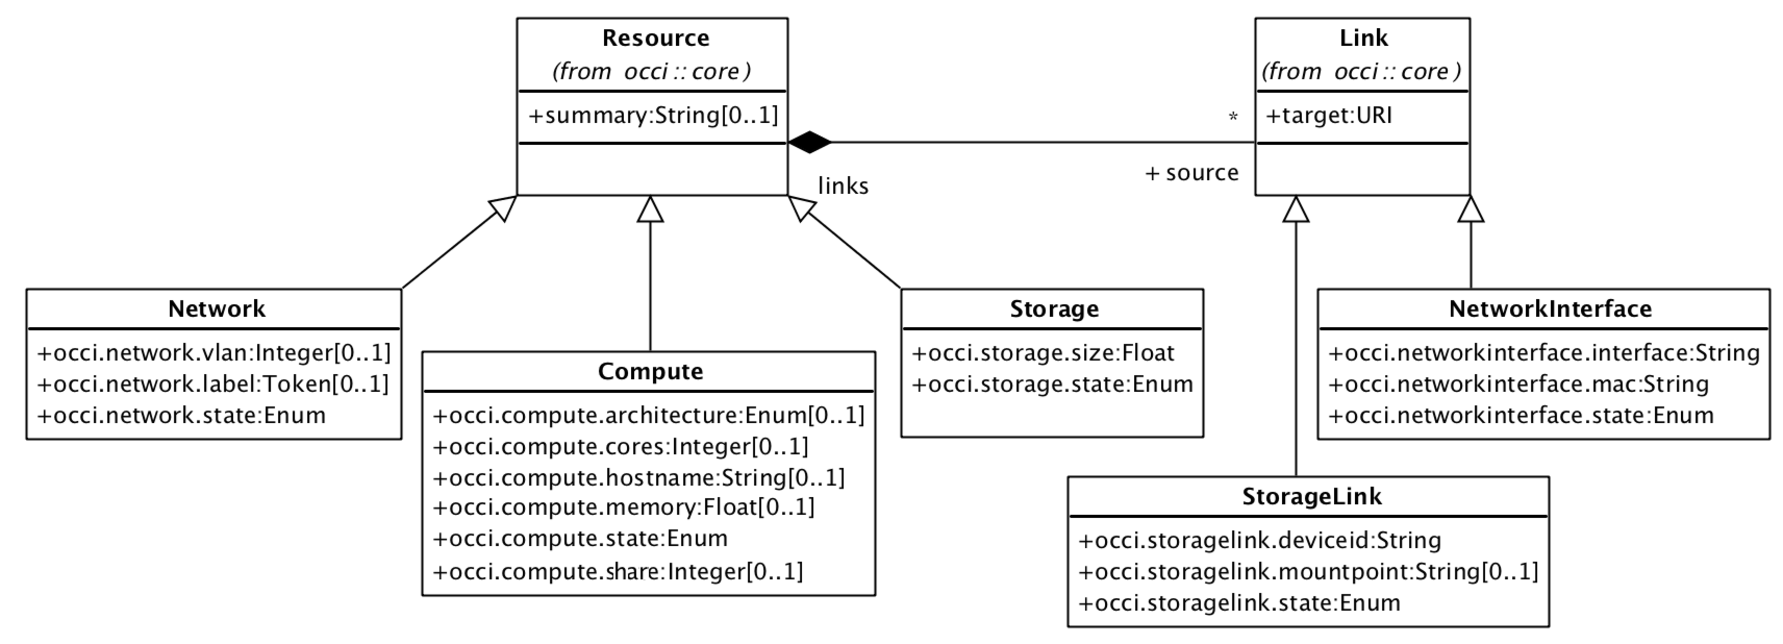
\includegraphics{figs/infrastructure_model.pdf}}} \par}
%	\caption{Overview Diagram of OCCI Infrastructure Types.}
%	\label{fig:infra_uml}
%\end{figure}


\subsection{The \smx\ mixin}

\mytablefloat{
	\label{tbl:smx}The immutable model attributes of the \smx\ mixin.
	The base URL {\bf http://schemas.ogf.org/occi} has been replaced with
	{\bf $<$schema$>$} in this table for a better reading experience. 
	} {
	\begin{tabular}{lllllll}
	\toprule
	Term & Scheme & Title & Attributes & Actions & Depends & Applies \\
	\colrule
	\smx &  $<$schema$>$/notification\# & \smx\ Mixin 
	& \{\} & \{\} & \{\} & $<$schema$>$/core\#Resource \\
	\botrule
	\end{tabular}
}

The {\em mixin} instance assigned to the \smx\ type is {\tt http://schemas.ogf.org/occi/notification\#notifier}, as in table \ref{tbl:smx}. The provider that supports the OCCI Notification extension MUST implement the \smx\ mixin for each provided entity kind.

There is no capability associated with the \smx\ mixin: it is a {\em tag}.

\subsection{The \ntfl\ link} 

\mytablefloat{
	\label{tbl:ntfl}The immutable model attributes of the \ntfl\ kind.
	The base URL {\bf http://schemas.ogf.org/occi} has been replaced with
	{\bf $<$schema$>$} in this table for a better readability experience. 
	} {
	\begin{tabular}{llllll}
	\toprule
	Term & Scheme & Title & Attributes & Actions & Parent \\
	\colrule
	\ntfl &  $<$schema$>$/notification\# & \ntfl\ Link
	& \{\} & \{\} & $<$schema$>$/core\#Link\\
	\botrule
	\end{tabular}
}

The {\em kind} instance assigned to the \ntfl\ type is {\tt http://schemas.ogf.org/occi/notification\#notification}, as in table \ref{tbl:ntfl}. The target of a \ntfl\ is a generic {\em Resource}, while the source MUST be associated with the \smx\ mixin. 

If the user requests the creation of a \ntfl\ whose source is not associated with a \smx\ mixin, the request MUST fail with an error.

If the user removes the \ntfl\ mixin associated with a {\em Resource}, all outgoing \ntfl\ links MUST be silently removed.

There is no capability associated with the \ntfl.

According with the core model \cite{occi:core}, the user is able to discover all \ntfl\ links that have their source in a given {\em Resource}.

According with the core model \cite{occi:core}, the removal of the source of an \ntfl\ link determines the removal of the link itself.

\section{Application notes and an example}

From the user perspective, the application of the \smx\ to a {\em Resource} corresponds to enabling the access to its state. This is significant mainly for {\em Resources} whose state changes in time.

The \smx\ mixin alone does not specify which changing aspect is in fact notified, and how: notably, not necessarily the attribute with {\sc state} id, if one exists. A further specification may be made explicit with a other mixins.

From the provider perspective the association of a \smx\ mixin is reflected in the implementation of the functionalities needed to observe and render the change. How this implemented depends on the {\em Resources} that are targets of the \ntfl.

The way in which notifications are used falls ouside the scope of this document: as a general rule, they are for management purposes. Such aspects can be defined by the user with mixins associated with the \ntfl\ link, or in the {\em Resource} targeted by the \ntfl.

The notification extension is inappropriate to describe the planned and periodic measurement of operational parameters of a resource for monitoring purposes: the monitoring extension \cite{occi:monitoring} specifically addresses such aspects, and may be coordinated with notification.

The following example (see figure \ref{fig:example}) illustrates a use case where the capabilities of the involved entities are implicit in the {\em Kind} of the target resource.

\begin{figure}
\centering
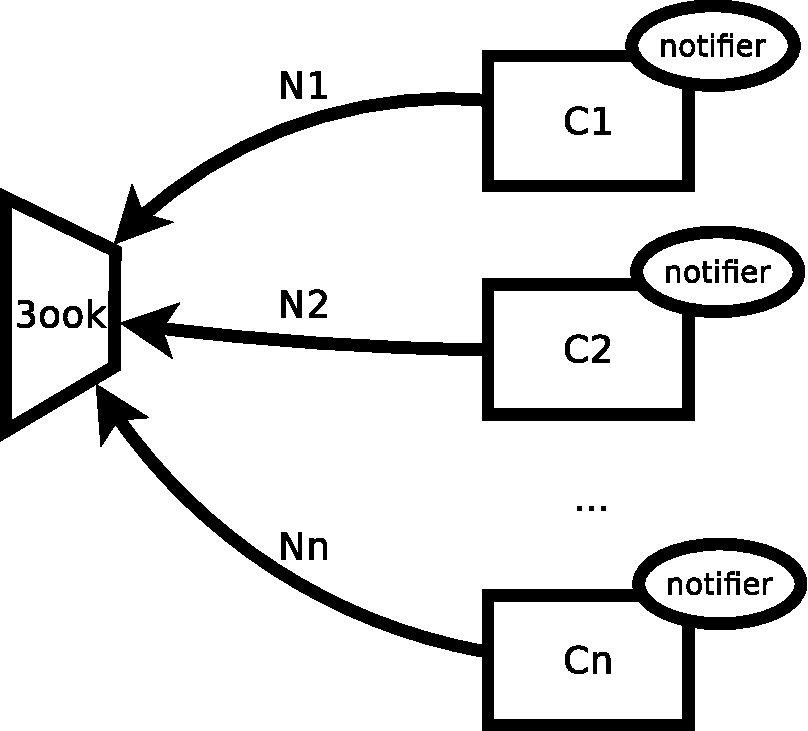
\includegraphics[width=0.3\textwidth]{figs/notificationExample.pdf}
\caption{Compute resources that notify their state to a control resource \label{fig:example}}
\end{figure}

\begin{quote}
A provider offers a Management Resource of {\em Kind} {\em 3-out-of-k}, that keeps in the {\em active} state 3 of the Compute resources from which it receives notifications.

The user that wants to take advantage of this service instantes a {\em 3-out-of-k} Resource $3ook$, and associates a \smx\ to each of the $k$ Compute resources $C_{1..k}$. For each of them a \ntfl\ link $N_i$ is instantiated that originates from $C_i$ and targets $3ook$.
\end{quote}

The schema is portable across any platform that offers the OCCI-infrastructure and OCCI-notification, and that provides a  {\em 3-out-of-k} {\em Kind}.

Distinct providers may interoperate, if an agreement exists that allows cross-provider information transfer: for instance, one provides the  {\em 3-out-of-k} Resource and another the Compute resources.

\section{Security issues}
The OCCI Notification specification is an extension to the OCCI Core
and Model specification \cite{occi:core}; thus the same security
considerations as for the OCCI Core and Model specification apply
here.

\section{Glossary}
\label{sec:glossary}
\todo{update glossary}

\begin{tabular}{l|p{12cm}}
Term & Description \\
\hline
\hl{Action} & An OCCI base type. Represents an invocable operation on a \hl{Entity} sub-type instance or collection thereof. \\

\hl{Attribute} & A type in the OCCI Core Model. Describes the name and properties of attributes found in \hl{Entity} types. \\

\hl{Category} & A type in the OCCI Core Model and the basis of the OCCI type identification mechanism. The parent type of \hl{Kind}. \\

capabilities & In the context of \hl{Entity} sub-types {\bf  capabilities} refer
  to the OCCI \hl{Attribute}s and OCCI \hl{Action}s exposed by an {\bf entity
  instance}. \\

\hl{Client} & An OCCI client.\\

\hl{Collection} & A set of \hl{Entity} sub-type instances all associated to a particular \hl{Kind} or \hl{Mixin} instance. \\

\hl{Entity} & An OCCI base type. The parent type of \hl{Resource} and \hl{Link}. \\

entity instance & An instance of a sub-type of \hl{Entity} but not an instance
  of the \hl{Entity} type itself.  The OCCI model defines two sub-types of
  \hl{Entity}, the \hl{Resource} type and the \hl{Link} type.  However, the
  term {\em entity instance} is defined to include any instance of a
  sub-type of \hl{Resource} or \hl{Link} as well. \\

\hl{Kind} & A type in the OCCI Core Model. A core component of the OCCI classification system. \\

\hl{Link} & An OCCI base type. A \hl{Link} instance associates one \hl{Resource} instance with another. \\

\hl{Mixin} & A type in the OCCI Core Model. A core component of the OCCI classification system. \\

mix-in & An instance of the \hl{Mixin} type associated with an {\em entity
 instance}. The ``mix-in'' concept as used by OCCI {\em only} applies to
 instances, never to \hl{Entity} types. \\

model attribute & An internal attribute of a the Core Model which is {\em not}
  client discoverable. \\

\hl{OCCI} & Open Cloud Computing Interface. \\

OCCI base type & One of \hl{Entity}, \hl{Resource}, \hl{Link} or \hl{Action}. \\

OCCI Action & see \hl{Action}. \\
OCCI Attribute & A client discoverable attribute identified by an instance of the \hl{Attribute} type. Examples are \hl{occi.core.title} and \hl{occi.core.summary}. \\
OCCI Category & see \hl{Category}. \\
OCCI Entity & see \hl{Entity}. \\
OCCI Kind & see \hl{Kind}. \\
OCCI Link & see \hl{Link}. \\
OCCI Mixin & see \hl{Mixin}. \\

OGF & Open Grid Forum. \\

\hl{Resource} & An OCCI base type. The parent type for all domain-specific \hl{Resource} sub-types. \\

resource instance & See {\em entity instance}. This term is considered obsolete. \\

tag & A \hl{Mixin} instance with no attributes or actions defined. \\

template & A \hl{Mixin} instance which if associated at instance
creation-time pre-populate certain attributes. \\

type & One of the types defined by the OCCI Core Model.  The Core Model types are
 \hl{Category}, \hl{Attribute},
 \hl{Kind}, \hl{Mixin}, \hl{Action}, \hl{Entity}, \hl{Resource}
 and \hl{Link}. \\

concrete type/sub-type & A concrete type/sub-type is a type that can be instantiated.\\

URI & Uniform Resource Identifier. \\
URL & Uniform Resource Locator. \\
URN & Uniform Resource Name. \\
\end{tabular}

 
%\section{Contributors}
%
We would like to thank the following people who contributed to this
document:

\begin{tabular}{l|p{2in}|p{2in}}
Name & Affiliation & Contact \\
\hline
Michael Behrens & R2AD & behrens.cloud at r2ad.com \\
Andy Edmonds & Intel - SLA@SOI project & andy at edmonds.be \\
Sam Johnston & Google & samj at samj.net \\
Gary Mazzaferro & OCCI Counselour - Exxia, Inc. &  garymazzaferro at gmail.com \\ 
Thijs Metsch & Platform Computing, Sun Microsystems & tmetsch at platform.com \\
Ralf Nyrén & Aurenav & ralf at nyren.net \\
Alexander Papaspyrou & TU-Dortmund & alexander.papaspyour at tu\-dortmund.de \\
Shlomo Swidler & Orchestratus & shlomo.swidler at orchestratus.com \\
\end{tabular}

Next to these individual contributions we value the contributions from
the OCCI working group.




\section{Intellectual Property Statement}
\input{include/ip}

\section{Disclaimer}
This document and the information contained herein is provided on an
``As Is'' basis and the OGF disclaims all warranties, express or
implied, including but not limited to any warranty that the use of the
information herein will not infringe any rights or any implied
warranties of merchantability or fitness for a particular purpose.


\section{Full Copyright Notice}
Copyright \copyright ~Open Grid Forum (2009-2016). All Rights Reserved.

This document and translations of it may be copied and furnished to
others, and derivative works that comment on or otherwise explain it
or assist in its implementation may be prepared, copied, published and 
distributed, in whole or in part, without restriction of any kind,
provided that the above copyright notice and this paragraph are
included as references to the derived portions on all such copies
and derivative works. The published OGF document from which such works
are derived, however, may not be modified in any way, such as by removing
the copyright notice or references to the OGF or other organizations,
except as needed for the purpose of developing new or updated OGF documents
in conformance with the procedures defined in the OGF Document Process,
or as required to translate it into languages other than English. OGF,
with the approval of its board, may remove this restriction for inclusion
of OGF document content for the purpose of producing standards in cooperation
with other international standards bodies. 

The limited permissions granted above are perpetual and will not be
revoked by the OGF or its successors or assignees.


\bibliographystyle{IEEEtran}
\bibliography{references}

\end{document}
